In this chapter we will explore the technical requirements for integrating \gls{rtcweb} with an enterprise communication system architecture and give the suggested solution along with discussing some of the problems raised by the integration.

\section{Integration}
There are basically two ways of going about this problem. The first would be to directly integrate \gls{wrtc} in the enterprise architecture. We could then use SIP-over-WebSocket signaling and use an end-to-end media path enabled by \gls{wrtc}. This could work if the legacy enterprise system supported all the required protocols defined in \gls{wrtc}, otherwise the architecture would have to be upgraded to support all the new features. This is not trivial, since it would require to redo all of the existing architecture just to support \gls{wrtc}. It is better to create a bridge in the form of a gateway between \gls{wrtc} and the legacy architecture.

\subsection{The Gateway}
First showing a simple web application P2P WebRTC structure. Here signaling goes through a signaling server and media travels directly between the two peers(browsers). A STUN server is used for receiving ICE candidates, if that fails there is a fallback transporting media through a TURN server.
\\
\begin{figure}[here]
\centerline{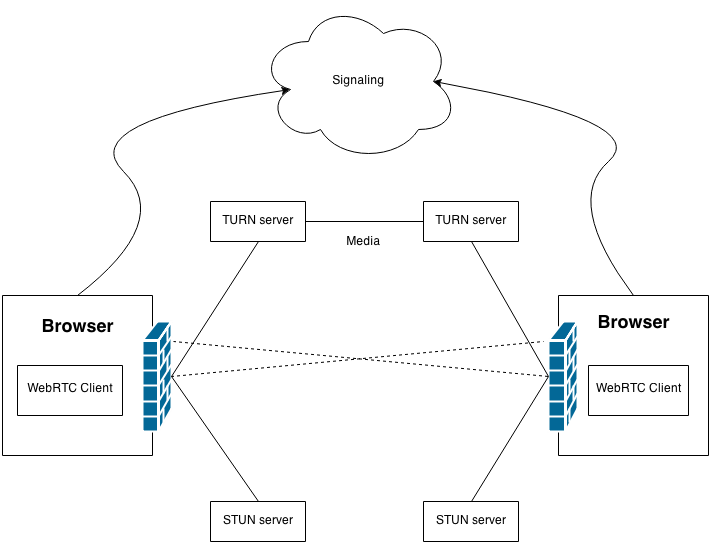
\includegraphics[scale=0.35]{webrtc-p2p-architecture.png}}
\caption{WebRTC P2P architecture}
\label{fig:jsep}
\end{figure}

Secondly showing a typical enterprise architecture with a signaling server, media server, and a server for routing the streams to peers.
\\
\begin{figure}[here]
\centerline{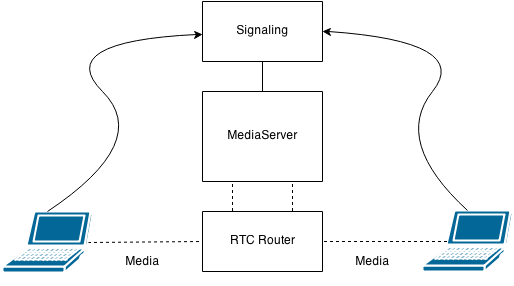
\includegraphics[scale=0.45]{enterprise-mcu-architecture.png}}
\caption{Enterprise communication platform architecture}
\label{fig:VirtualArenaArchitecture}
\end{figure}

Let's see how RTCWeb can be used to connect to existing enterprise communication networks. In the solution figure we add an interworking gateway component. This component includes three subcomponents:

\begin{itemize}
\item{Signaling Proxy}
\item{Media Transport Proxy}
\item{Media Transcoder}
\end{itemize}

These components should provide all the necessary functionality we need.
\\
\begin{figure}[here]
\centerline{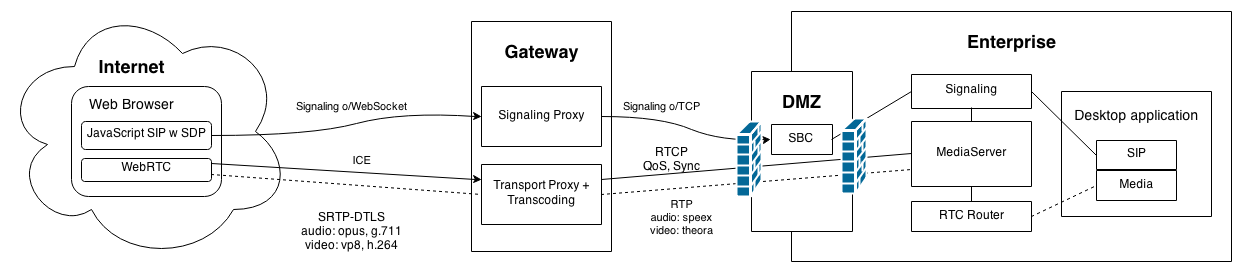
\includegraphics[scale=0.40]{gateway2.png}}
\caption{WebRTC-Enterprise Gateway}
\label{fig:wrtc-enterprise-gateway}
\end{figure}

\subsection{The Signaling Proxy}
In this implemenation the client has implemented signaling using a \gls{sip} stack in Javascript. The SIP includes the \gls{sdp} and this is transmitted over HTTP using WebSockets. Then the signaling proxy will manipulate the \gls{sdp} to support the enterprise implementation of \gls{sip} or any other proprietary way. The SDP would also only include TURN addresses so we make sure that the media always gets routed through th e gateway, blocking all other candidates. The message would then be transported through the enterprise \gls{sbc}. The Signaling proxy has to generate an offer for the client, then on the client the remote party would install it using the setRemoteDescription() API.

\subsection{The Transport Proxy}
The \gls{wrtc} specification make support for \gls{ice} and \gls{srtp}-{dtls} mandatory. The problem here is that our enterprise architecture uses raw \gls{rtp} streams, it does not need the added transport layer security that \gls{wrtc} defines, becuse of its strict firewall policies. It is up to the Transport Proxy to convert the media streams to allow these two worlds to interoperate. The Transport Proxy also has to function like a TURN server, this so we can route the media through our gateway. The Transport Proxy handles the ICE connectivity checks, which in this case would only serve the address of our Transport Proxy. We do this by modifying a constraint in the IceTransport object on the client.

\subsection{The Media Transcoder}
The \gls{wrtc} specification defines these mandatory codecs:
\begin{itemize}
    \item Audio: opus and g.711
    \item Video: ?
\end{itemize}

There are still discussions on the topic of which video codec should be standard. The choice is between VP8 and H.264. The H.264 codec was recently made free by Cisco, so now both choices are royalty free. H.264 is the most widely deployed and currently has the best hardware support, but both Google and Firefox has decided to use VP8 in their WebRTC implementations. However, the Bowser browser created by ericsson for iOS, has only implemented support for h.264 in their WebRTC solution.

Our enterprise applicaton uses Speex for audio and Theora for video. So these would have to be transcoded to the appropriate formats. This is one of the advantages of creating a media transcoder because you can add support for both H.264 and VP8 and be able to create a session between Chrome, our enterprise software, and the Bowser browser on iOS. Problem with this component is that it's expensive in terms of processing and it may cause some delays in the stream.

\section{Summary}
The first iteration of RTCWeb is still under development, and not all protocols and codecs have been decided yet. It is theoretically possible to create a gateway and it has been done before under closed doors for similar systems. Some of the biggest issues are how to handle the signaling, translating the media, and crossing the enterprise firewall. The interworking efforts at the media level are expensive, and \gls{sdp} handling can be quite complex, as it will probably require remapping of its properties.